\documentclass{shortart}

\usepackage{amsmath, amssymb, amsthm}
\usepackage{tikz}
\usepackage{tikz-cd}
\usepackage{plastex}

\title{The Barratt--Priddy--Quillen--Segal theorem}
\author{Dexter Chua}

\newtheorem{lemma}{Lemma}
\newtheorem{thm}[lemma]{Theorem}
\newtheorem{prop}[lemma]{Proposition}
\newtheorem*{claim}{Claim}

\theoremstyle{definition}
\newtheorem{defi}[lemma]{Definition}
\newtheorem{eg}[lemma]{Example}

\DeclareMathOperator\Cob{Cob}
\DeclareMathOperator\Conf{Conf}
\newcommand\A{\mathbb{A}}
\newcommand\E{\mathbb{E}}
\newcommand\N{\mathbb{N}}
\newcommand\R{\mathbb{R}}
\newcommand\gp{\mathrm{gp}}

\newcommand\dcirc[1]{\node [fill, circle, inner sep = 0, minimum size = 3] at #1 {};}

\begin{document}

The goal of this talk is to understand the ``moduli space of $0$-dimensional (compact) manifolds''. Of course, $0$-dimensional manifolds are not very interesting. They are just a finite collection of points. The diffeomorphism classes of $0$-dimensional manifolds are indexed by the natural numbers $\N$, and the automorphism group of $[n]$ is $\Sigma_n$. So the (homotopy type of) the moduli space is
\[
  \mathcal{M} = \coprod_{n \geq 0} B \Sigma_n.
\]

The disjoint union of manifolds endows $\mathcal{M}$ with the structure of an $\A_\infty$-monoid. This is the correct notion of a topological monoid in the homotopical setting. It is in fact $\E_\infty$, but we shall focus on the $\A_\infty$ structure. We will provide a concrete definition of an $\A_\infty$-monoid later on and explicitly describe this $\A_\infty$ structure.

If $X$ is any $\A_\infty$-monoid, then $\pi_0(X)$ is a monoid, which may or may not be a group. We say $X$ is group-like (or an $\A_\infty$-group) if $\pi_0(X)$ is a group, and the group completion of $X$, written $X \to X^{\gp}$, is the universal map of $\A_\infty$-monoids from $X$ to an $\A_\infty$-group. In the previous talk, we discussed the group completion theorem, which relates the homology of $X^\gp$ to that of $X$.

\begin{thm}
  There is an equivalence of $\A_\infty$-groups
  \[
    \mathcal{M}^{\gp} \overset{\sim}{\to} \lim_{N \to \infty} \Omega^N S^N.
  \]
\end{thm}

There is an ``easy'' abstract nonsense proof of this theorem --- simply observe that both sides are the free $\E_\infty$-group on a point. However, the perspective we want to take is that $\mathcal{M}$ is the moduli of $0$-dimensional manifolds, and so we want a proof that adopts this perspective.

In this talk, we will construct an explicit geometric model of $\mathcal{M}$ and endow it with the structure of an $\A_\infty$-monoid. We will then use this explicit model to prove the equivalence above.

First of all, instead of thinking about ``all'' $0$-dimensional manifolds, we consider $0$-dimensional submanifolds of $\R^\infty$. In general,

\begin{defi}
  If $M$ is a manifold, write $\Conf_n(M)_{\Sigma_n}$ for the space of $n$ distinct (unordered) points on $M$.
\end{defi}

We define
\[
  \Conf_n(\R^\infty)_{\Sigma_n} = \lim_{N \to \infty} \Conf_n(\R^N)_{\Sigma_n}.
\]
It is not difficult to see that this is a model of $B \Sigma_n$, using the fact that the space of embeddings of $n$ points in $\R^N$ is $\sim N$ connected. So we have
\[
  \mathcal{M} = \lim_{N \to \infty} \coprod_{n \geq 0} \Conf_n(\R^N)_{\Sigma_n}
\]

It will be useful to consider a variant of this configuration space:
\begin{defi}
  $C(\R^N)$ is the set of discrete subsets of $\R^N$, where a sequence of configurations converges if the intersection with any open ball converges.
\end{defi}
To get a feel of what this space is like, we can describe some properties of it. For example this space is path connected, because given any configuration, we can push all points out to infinity to get a path to $\emptyset$. In fact, we can explicitly describe the homotopy type.

\begin{prop}
  $C(\R^N) \simeq S^N$.
\end{prop}

\begin{proof}
  We shall define two contractible open subsets $U_0, U_1 \subseteq C(\R^N)$ such that $U_0 \cap U_1 \simeq S^{N - 1}$. Then we have a homotopy pushout square
  \begin{useimager}
    \[
      \begin{tikzcd}
        U_0 \cap U_1 \ar[r] \ar[d] & U_0\ar[d]\\
        U_1 \ar[r] & C(\R^N)
      \end{tikzcd}
    \]
  \end{useimager}
  that exhibits $C(\R^N)$ as the suspension of $S^{N - 1}$, hence is $S^N$.

  We define the subsets $U_0, U_1$ as follows:
  \begin{itemize}
    \item $U_0$ contains the configurations with no point at the origin. 
    \item $U_1$ contains the configurations with a unique point closest to the origin.
  \end{itemize}
  These indeed cover --- if a configuration is not in $U_0$, then it contains a point at the origin, which is necessarily the unique point closest to the origin. We observe
  \begin{itemize}
    \item $U_0$ deformation retracts to $\emptyset$ by pushing every point away from the origin;
    \item $U_1$ deformation retracts to $\{(0, 0)\}$ by translating the distinguished point to the origin, then pushing all other points out to infinity;
    \item $U_0 \cap U_1$ deformation retracts onto $S^{N - 1}$ by scaling the distinguished point to radius $1$, then pushing all other points to infinity.\qedhere
  \end{itemize}
\end{proof}

We generalize the definition of $C(\R^N)$ a bit:
\begin{defi}
  If $U \subseteq \R^N$ is open, we define $C(U)$ to be the subset of $C(\R^N)$ consisting of the configurations that are contained in $U$.
\end{defi}

\begin{eg}
  If $I$ is the interval $[0, 1]$, then
  \[
    C(I^N) \cong \coprod_{n \geq 0} \Conf_n(I^N)_{\Sigma_n} \cong \coprod_{n \geq 0} \Conf_n(\R^N)_{\Sigma_n}.
  \]
  So
  \[
    \mathcal{M} \cong \lim_{N \to \infty} C(I^N).
  \]
\end{eg}

The main theorem we have to prove is the following:
\begin{thm}
  Let $U \subseteq \R^N$ be an open subspace of the form $\R^k \times V$ with $V$ precompact. Then $C(I \times U)$ has a canonical structure as an $\A_\infty$-monoid and
  \[
    C(I \times U)^\gp \simeq \Omega C(\R \times U).
  \]
  Iterating this with the case $U = \R^k \times I^j$, we find that
  \[
    \mathcal{M}^{\gp} \cong \lim_{N \to \infty} \Omega^N C(\R^N) = \lim_{N \to \infty} \Omega^N S^N.
  \]
\end{thm}
It is reasonable to expect the theorem to be true for more general $U$, but I only know of a proof for $U$ of this particular form.

The idea of the theorem is that if $C(I \times U)$ were a topological monoid, then the theorem is equivalent to $B C(I \times U) \cong C(R \times U)$, and in the bar construction for $C(I \times U)$, we have lots of copies of $I$ put next to each other, which give us an $\R$.

To actually prove the theorem, we need to first know what it means to be an $\A_\infty$-monoid. It turns out the definition of an $\A_\infty$-monoid is one such that the idea above can be made literally true.

Our notion of an $\A_\infty$-monoid is what people call a reduced Segal space. The idea is that a reduced Segal space is a simplicial space that ``looks like'' the bar resolution of a topological monoid.

\begin{defi}
  An $\A_\infty$-monoid is a (proper) simplicial space $X_\bullet$ such that the maps $X_p \to X_1^p$ given by the inclusions $[1] \hookrightarrow [p]$ sending $\{0, 1\} \mapsto \{i, i + 1\}$ is a weak equivalence. In particular, $X_0 \simeq *$.
\end{defi}

Given an $\A_\infty$-monoid $X_{\bullet}$, we will refer to $X_1$ as the underlying space, and we expect the geometric realization $\|X_\bullet\|$ to be the delooping of $X_1$. The main theorem (whose proof we omit) is the following:
\begin{thm}
  If $X_\bullet$ is an $\A_\infty$-monoid, then $X_1^\gp \cong \Omega \|X_\bullet\|$.\fakeqed
\end{thm}

So to prove the main theorem, we need to construct $X_\bullet$ such that $X_1 \cong C(I \times U)$ and $\|X_\bullet\| \cong C(\R \times U)$.
\begin{proof}[Proof of main theorem]
  We define $X_p$ to be the subset of $C(\R \times U) \times \R^{p + 1}$ consisting of elements $(\mathbf{x}, t_0 \leq \cdots \leq t_p)$ such that $\mathbf{x}$ never meets the ``walls'' $\{t_i\} \times U$. The face map $d_i$ forgets the wall $t_i$,  and the degeneracies repeat the corresponding wall.\footnote{Na\"ively, one might think we should require the points to lie within $(t_0, t_p) \times U$. It gives the same homotopy type because we can push the outside points away to infinity, but our formulation here makes the proof go more smoothly.}

  \begin{center}
    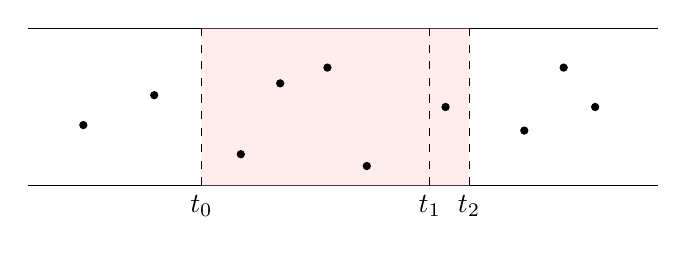
\begin{tikzpicture}
     \draw (-4, 0) -- (4, 0);
     \draw (-4, 2) -- (4, 2);

     \fill [opacity=0.3, pink] (-1.8, 0) rectangle (1.6, 2);

     \draw [dashed] (-1.8, 0) node [below] {$t_0$} -- +(0, 2);
     \draw [dashed] (1.1, 0) node [below] {$t_1$} -- +(0, 2);
     \draw [dashed] (1.6, 0) node [below] {$t_2$} -- +(0, 2);

     \dcirc{(-1.3, 0.4)}
     \dcirc{(-0.2, 1.5)}
     \dcirc{(1.3, 1)}
     \dcirc{(0.3, 0.25)}
     \dcirc{(-0.8, 1.3)}
     \dcirc{(2.3, 0.7)}
     \dcirc{(2.8, 1.5)}
     \dcirc{(3.2, 1)}
     \dcirc{(-3.3, 0.77)}
     \dcirc{(-2.4, 1.15)}
    \end{tikzpicture}
  \end{center}

  There is an inclusion $C(I \times U) \cong C(I \times U) \times \{(0, 1)\} \hookrightarrow X_1$, which is a deformation retract, and in particular a homotopy equivalence. This deformation retract is simply given by scaling the $t_i$ the configuration and $t_i$ linearly until $(t_0, t_1) = (0, 1)$, and then pushing the points with $t \not\in (0, 1)$ away to infinity. Similarly, we get $X_p \simeq C(I \times U)^p$ and we see that $X_\bullet$ is indeed an $\A_\infty$-monoid.

  We next need to show that $\|X_\bullet\| \simeq C(\R \times U)$. A point in $\|X_\bullet\|$ is an element $(\mathbf{x}, t_0 < \cdots < t_p)$ together with some non-zero weights on the $t_i$ summing to $1$, modulo some equivalence relations. We define a map $p: \|X_\bullet\| \to C(\R \times U)$ that simply forgets the walls and weights.

  We first prove that this is a weak equivalence if $U$ is precompact. The strategy is to show that this map is a Serre microfibration with weakly contractible fibers. Recall that a Serre fibration is a map $A \to B$ where we can always solve the lifting problem
  \begin{useimager}
    \[
      \begin{tikzcd}
        D^k \ar[d] \ar[r] & A \ar[d]\\
        D^k \times [0, 1] \ar[r] \ar[ur, dashed] & B
      \end{tikzcd}
    \]
  \end{useimager}
  A Serre microfibration is a weaker notion where we only need to be able to lift of the restriction of the bottom map to $D^k \times [0, \varepsilon)$ for some small $\varepsilon > 0$. It is a theorem that a Serre microfibration with weakly contractible fibers is a weak equivalence.

  The map is easily seen to be a microfibration in the case where $U$ is precompact, because any element in $C(I \times U)$ only has finitely many points and so the configuration of points is bounded away from the walls, so any small perturbation of the points will still not hit the walls. If $U$ is not precompact, this argument fails because we can have infinitely many points that can get arbitrarily close to the walls, and we need to modify our argument.

  To see that the fibers are contractible, fix $\mathbf{x} \in C(\R \times U)$. Then $p^{-1}(\{\mathbf{x}\})$ is the space of ways to insert walls and weights that do not hit $\mathbf{x}$. If $K$ is a compact space and $f: K \to p^{-1}(\{\mathbf{x}\})$ is a map, then by compactness, the walls in $f(K)$ are bounded. So we can pick a $T$ so large that the walls in $f(K)$ are all $ < T$, and we may also assume $\{T\} \times U$ does not hit $\mathbf{x}$. There is then a homotopy from $f$ to the constant map on $(\mathbf{x}, T)$ by scaling down the weights at the existing walls and putting the weights on $T$. So $p^{-1}(\{\mathbf{x}\})$ is contractible.

  In the case where $U \cong \R^k \times V$ is not precompact, we have to do a bit more work. We define another space $X'_\bullet$ whose $p$-simplices is the subspace of $C(\R \times U) \times \R^{p + 1} \times (\R^k)^{p + 1}$ consisting of $(\mathbf{x}, t_0 \leq \ldots \leq t_p, y_0, \ldots, y_p)$ such that $\mathbf{x}$ is disjoint from the subset $\{t_i\} \times \{y_i\} \times V \subseteq \R \times \R^k \times V$ of the wall (and we require $y_i = y_j$ if $t_i = t_j$). This is a \emph{less} restrictive condition, and we have maps
  \begin{useimager}
    \[
      \begin{tikzcd}[column sep=small]
        \|X_\bullet\| \ar[rr] \ar[rd, "p"'] & & \|X_\bullet'\| \ar[ld, "p'"]\\
        & C(\R \times U)
      \end{tikzcd}
    \]
  \end{useimager}
  The horizontal map sets $y_i = 0$ and is a deformation retract because we can push points on $\{t_i\} \times \R^k \times V$ away from the point $y_i$ (and then translate $y_i$ to $0$). Then the above argument generalizes to show that $p'$ is a Serre microfibration with weakly contractible fibers.

  \begin{center}
    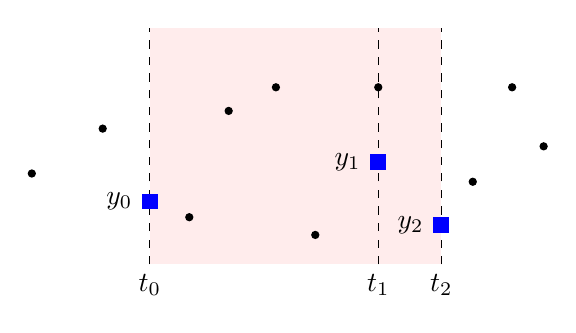
\begin{tikzpicture}
      \begin{scope}[yscale=1.5]
        \fill [opacity=0.3, pink] (-1.8, 0) rectangle (1.9, 2);

        \draw [dashed] (-1.8, 0) node [below] {$t_0$} -- +(0, 2);
        \draw [dashed] (1.1, 0) node [below] {$t_1$} -- +(0, 2);
        \draw [dashed] (1.9, 0) node [below] {$t_2$} -- +(0, 2);

        \dcirc{(-1.3, 0.4)}
        \dcirc{(-0.2, 1.5)}
        \dcirc{(1.1, 1.5)}
        \dcirc{(0.3, 0.25)}
        \dcirc{(-0.8, 1.3)}
        \dcirc{(2.3, 0.7)}
        \dcirc{(2.8, 1.5)}
        \dcirc{(3.2, 1)}
        \dcirc{(-3.3, 0.77)}
        \dcirc{(-2.4, 1.15)}
      \end{scope}

      \fill [blue] (-1.9, 0.7) rectangle +(0.2, 0.2);
      \node [left] at (-1.9, 0.8) {$y_0$};

      \fill [blue] (1.0, 1.2) rectangle +(0.2, 0.2);
      \node [left] at (1.0, 1.3) {$y_1$};

      \fill [blue] (1.8, 0.4) rectangle +(0.2, 0.2);
      \node [left] at (1.8, 0.5) {$y_2$};
    \end{tikzpicture}
  \end{center}\qedshift
\end{proof}

This proof is meant to serve as a blueprint for understanding the moduli space of higher dimensional manifolds. In the positive dimensional case, essentially the same proof will show that (the classifying space of) the ``cobordism category'' is homotopy equivalent to an explicit infinite loop space. The main differences are as follows:
\begin{enumerate}
  \item We have to relate this cobordism category to the moduli space of manifolds. In the $0$-dimensional case, this requires almost no work. Indeed, we managed to avoid mentioning the cobordism category at all.
  \item We have to identify the replacement of $C(\R^n)$ with an appropriate Thom space. This will be done with a technique known as scanning.
  \item One has to put some effort into defining the right topology on the moduli spaces, which is more complicated than the zero-dimensional case. In the $0$-dimensional case, we had this trick of considering the space $X_\bullet'$ in addition to $X_\bullet$, and in positive dimensions, we need to play multiple similar tricks to relate different models of the moduli space.
\end{enumerate}
\end{document}
